\documentclass{beamer}
\usepackage{multicol}  % for multiple columns
\usepackage{etoolbox}  % for toggles
\usepackage{subcaption}
%\usepackage{fancyvrb}
\usepackage{listings} % for colored verbatim
% required packages
\usepackage{xcolor}
\usepackage{stmaryrd} % jump brackets: \llbracket, \rrbracket

% create a provideenvironment command
\makeatletter
\def\provideenvironment{\@star@or@long\provide@environment}
\def\provide@environment#1{%
  \@ifundefined{#1}%
    {\def\reserved@a{\newenvironment{#1}}}%
    {\def\reserved@a{\renewenvironment{dummy@environ}}}%
  \reserved@a
}
\def\dummy@environ{}
\makeatother

% directories
\newcommand{\diagramdirectory}{../diagrams}

% general
\newcommand{\x}{\mathbf{x}}
\newcommand{\qpoint}{\x_q}
\newcommand{\timevalue}{t}
\newcommand{\timestepsize}{\Delta\timevalue}
\newcommand{\dt}{\timestepsize}
\newcommand{\timeindex}{n}
\newcommand{\speed}{v}
\newcommand{\velocity}{\mathbf{\speed}}
\newcommand{\velocityx}{u}
\newcommand{\velocityy}{v}
\newcommand{\velocityn}{v_n}
\newcommand{\vx}{\velocityx}
\newcommand{\vy}{\velocityy}
\newcommand{\vn}{\velocityn}

% normal vector
\newcommand{\normalvectorletter}{n}
\newcommand{\normalvector}{\mathbf{\normalvectorletter}}
\newcommand{\normalx}{\normalvectorletter_x}
\newcommand{\normaly}{\normalvectorletter_y}
\newcommand{\nx}{\normalx}
\newcommand{\ny}{\normaly}

\newcommand{\ndimensions}{N_\text{dim}}
\newcommand{\ncomponents}{m}
\newcommand{\ndofs}{N_\text{dof}}
\newcommand{\nnodes}{N_\text{node}}
\newcommand{\dofindex}{j}
\newcommand{\nodeindex}{k}
\newcommand{\componentindex}{k}
\newcommand{\transpose}{^{\text{T}}}

% schemes
\newcommand{\low}{L}
\newcommand{\high}{H}

% solution
\newcommand{\scalarsolution}{u}
\newcommand{\vectorsolution}{\mathbf{\scalarsolution}}
\newcommand{\approximate}[1]{\tilde{#1}}
\newcommand{\approximatescalarsolution}{\approximate{\scalarsolution}}
\newcommand{\approximatevectorsolution}{\approximate{\vectorsolution}}
\newcommand{\solutionletter}{U}
\newcommand{\solutionvector}{\mathbf{\solutionletter}}
\newcommand{\U}{\solutionvector}
\newcommand{\lowordersolution}[1][]{
  \ifthenelse{\equal{#1}{}}{\solutionvector^L}{\solutionvector^{L,#1}}}
\newcommand{\highordersolution}[1][]{
  \ifthenelse{\equal{#1}{}}{\solutionvector^H}{\solutionvector^{H,#1}}}

% math
\newcommand{\triangulation}{\mathcal{K}_h}
\newcommand{\approximationspace}{\mathcal{U}_h}
\newcommand{\approximationspaceinc}{\approximationspace^{\textup{inc}}}
\newcommand{\referenceelementmap}{\Phi}
\newcommand{\qonespace}{\mathbb{Q}_1}

% sets
\newcommand{\faces}{\mathcal{F}}
\newcommand{\quadraturepoints}{\mathcal{Q}}

% domain and FEM
\newcommand{\domain}{\mathcal{D}}
\newcommand{\celldomain}[1][\cell]{\domain_#1}
\newcommand{\facedomain}{\domain}
\newcommand{\domainboundary}{\partial\domain}
\newcommand{\incomingdomainboundary}{\domainboundary^{\textup{inc}}}
\newcommand{\cellindex}{K}
\newcommand{\cell}{K}
\newcommand{\celldiameter}{\Delta x}
\newcommand{\maxcelldiameter}{\Delta x_{\text{max}}}
\newcommand{\volume}{V}
\newcommand{\dvolume}{\,d\x}
\newcommand{\area}{A}
\newcommand{\darea}{\,d\area}
\newcommand{\testfunction}{\varphi}
\newcommand{\vectortestfunctionscalar}{\Phi}
\newcommand{\vectortestfunction}{\mathbf{\vectortestfunctionscalar}}
\newcommand{\support}{S}
\newcommand{\maxdof}{N}
\newcommand{\interpolant}{\Pi}

% local viscous bilinear form
\newcommand{\localvisc}{b}
\newcommand{\localviscbilinearform}[3]{\localvisc_#1(\testfunction_#2, \testfunction_#3)}
\newcommand{\cellvolume}{|\celldomain|}
\newcommand{\cardinality}[1][]{\ifthenelse{\equal{#1}{}}{n_\cell}{n_#1}}
\newcommand{\cardsystem}{\bar{n}}
\newcommand{\indices}{\mathcal{I}}
\newcommand{\cellindices}{\mathcal{K}}
\newcommand{\indicesnode}{\indices^{\text{node}}_\cell}
\newcommand{\indicescell}[1][]{\ifthenelse{\equal{#1}{}}{\indices_\cell}
  {\indices_{#1}}}
\newcommand{\incomingindices}{\indices^{\textup{inc}}}
\newcommand{\notincomingindices}{\indices(\triangulation)\setminus\incomingindices}

% entropy viscosity
\newcommand{\entropy}{\eta}
\newcommand{\entropyflux}{\mathbf{\consfluxletter}^\eta}
\newcommand{\entropyjump}{\mathcal{J}}
\newcommand{\entropyresidual}{\mathcal{R}}
\newcommand{\entropyresidualcoef}{c_\entropyresidual}
\newcommand{\entropyjumpcoef}{c_\entropyjump}
\newcommand{\entropynormalization}{\hat{\entropy}}

% conservation law
\newcommand{\consfluxletter}{f}
\newcommand{\consflux}{\mathbf{\consfluxletter}}
\newcommand{\consfluxsystem}{\mathbf{\MakeUppercase{\consfluxletter}}}
\newcommand{\consfluxscalar}[1][\scalarsolution]{\mathbf{\consfluxletter}(#1)}
\newcommand{\consfluxvector}{\mathbf{\MakeUppercase{\consfluxletter}}}
\newcommand{\consfluxvectory}{\mathbf{G}}
\newcommand{\consfluxvectorn}{\consfluxvector_{n}}
\newcommand{\consfluxinterpolant}{\mathrm{F}}
\newcommand{\conssource}{\mathbf{s}}

% viscosity
\newcommand{\viscosity}{\nu}
\newcommand{\cellviscosity}{\viscosity_\cellindex}
\newcommand{\lowordercellviscosity}[1][]{
  \ifthenelse{\equal{#1}{}}{\cellviscosity^L}
  {\cellviscosity^{L,#1}}}
\newcommand{\highordercellviscosity}[1][]{
  \ifthenelse{\equal{#1}{}}{\cellviscosity^H}
  {\cellviscosity^{H,#1}}}
\newcommand{\entropycellviscosity}[1][]{
  \ifthenelse{\equal{#1}{}}{\cellviscosity^\entropy}
  {\cellviscosity^{\entropy,#1}}}

% viscous fluxes
\newcommand{\viscstring}{\text{visc}}
\newcommand{\viscflux}[1]{\mathbf{\consfluxletter}^{\viscstring,#1}}
\newcommand{\viscconsfluxvector}
  {\mathbf{\MakeUppercase{\consfluxletter}}^\viscstring
  (\vectorsolution,\viscosity)}

% mass matrix
\newcommand{\massmatrixletter}{M}
\newcommand{\massmatrix}{\mathbf{\massmatrixletter}}
\newcommand{\M}{\massmatrix}
\newcommand{\consistentmassmatrix}{\massmatrix^C}
\newcommand{\consistentmassentry}{\massmatrixletter^C_{i,j}}
\newcommand{\lumpedmassmatrix}{\massmatrix^L}
\newcommand{\lumpedmassentry}{\massmatrixletter^L_{i,i}}

% gradient matrix (for conservation law systems)
\newcommand{\gradientmatrixletter}{c}
\newcommand{\gradientmatrix}{\mathbf{\MakeUppercase{\gradientmatrixletter}}}
\newcommand{\gradiententry}{\mathbf{\gradientmatrixletter}\ij}

% steady-state system matrix and rhs
\newcommand{\ssmatrixletter}{A}
\newcommand{\ssmatrix}[1][]{
  \ifthenelse{\equal{#1}{}}
  {\mathbf{\ssmatrixletter}}
  {\mathbf{\ssmatrixletter}^#1}}
\newcommand{\A}{\ssmatrix}
\newcommand{\loworderssmatrix}[1][]{
  \ifthenelse{\equal{#1}{}}
  {\ssmatrix^L}
  {\ssmatrix^{L,#1}}}
\newcommand{\highorderssmatrix}[1][]{
  \ifthenelse{\equal{#1}{}}
  {\ssmatrix^H}
  {\ssmatrix^{H,#1}}}
\newcommand{\ssrhsletter}{b}
\newcommand{\ssrhs}[1][]{
  \ifthenelse{\equal{#1}{}}
  {\mathbf{\ssrhsletter}}
  {\mathbf{\ssrhsletter}^#1}}
\renewcommand{\b}{\ssrhs}
\newcommand{\ssresletter}{r}
\newcommand{\ssres}{\mathbf{\ssresletter}}
\renewcommand{\r}{\ssres}
\newcommand{\B}{\mathbf{B}}
\newcommand{\s}{\mathbf{s}}

% diffusion matrix
\newcommand{\diffusionmatrixletter}{D}
\newcommand{\diffusionmatrix}[1][]{
  \ifthenelse{\equal{#1}{}}
  {\mathbf{\diffusionmatrixletter}}
  {\mathbf{\diffusionmatrixletter}^#1}}
\newcommand{\D}{\diffusionmatrix}
\newcommand{\loworderdiffusionmatrix}[1][]{
  \ifthenelse{\equal{#1}{}}
  {\diffusionmatrix^L}
  {\diffusionmatrix^{L,#1}}}
\newcommand{\highorderdiffusionmatrix}[1][]{
  \ifthenelse{\equal{#1}{}}
  {\diffusionmatrix^H}
  {\diffusionmatrix^{H,#1}}}

% Runge-Kutta
\newcommand{\RKstagesolution}{\hat{\mathbf{\solutionletter}}}
\newcommand{\RKintermediatesolution}{\tilde{\mathbf{\solutionletter}}}
\newcommand{\RKoldsolutioncoef}{\alpha}
\newcommand{\RKstagesolutioncoef}{\beta}
\newcommand{\RKtimecoef}{c}
\newcommand{\RKstagetime}{\hat{\timevalue}}
\newcommand{\RKnstages}{s}

% FCT
\newcommand{\solutionbound}{W}
\newcommand{\DMPlowerbound}{\solutionbound^{\textup{DMP},-}}
\newcommand{\DMPupperbound}{\solutionbound^{\textup{DMP},+}}
\newcommand{\DMPlowerboundss}{\solutionbound^{\textup{DMP},\textup{ss},-}}
\newcommand{\DMPupperboundss}{\solutionbound^{\textup{DMP},\textup{ss},+}}
\newcommand{\DMPboundsss}{\solutionbound^{\textup{DMP},\textup{ss},\pm}}
\newcommand{\DMPlowerboundee}{\solutionbound^{\textup{DMP},\textup{ee},-}}
\newcommand{\DMPupperboundee}{\solutionbound^{\textup{DMP},\textup{ee},+}}
\newcommand{\DMPboundsee}{\solutionbound^{\textup{DMP},\textup{ee},\pm}}
\newcommand{\DMPlowerboundtheta}{\solutionbound^{\textup{DMP},\textup{theta},-}}
\newcommand{\DMPupperboundtheta}{\solutionbound^{\textup{DMP},\textup{theta},+}}
\newcommand{\DMPboundstheta}{\solutionbound^{\textup{DMP},\textup{theta},\pm}}
\newcommand{\DMPbounds}{\solutionbound^{\textup{DMP},\pm}}
\newcommand{\analyticDMPbounds}{\solutionbound^{\textup{analytic},\pm}}
\newcommand{\analyticDMPupperbound}{\solutionbound^{\textup{analytic},+}}
\newcommand{\analyticDMPlowerbound}{\solutionbound^{\textup{analytic},-}}
\newcommand{\limitedfluxbound}{Q}
\newcommand{\antidiffusionbound}{\limitedfluxbound}
\newcommand{\antidiffusionboundvector}{\mathbf{\limitedfluxbound}}
\newcommand{\antidiffusionlowerboundss}{\antidiffusionbound^{\textup{ss},-}}
\newcommand{\antidiffusionupperboundss}{\antidiffusionbound^{\textup{ss},+}}
\newcommand{\antidiffusionlowerboundee}{\antidiffusionbound^{\textup{ee},-}}
\newcommand{\antidiffusionupperboundee}{\antidiffusionbound^{\textup{ee},+}}
\newcommand{\antidiffusionlowerboundtheta}{\antidiffusionbound^{\textup{theta},-}}
\newcommand{\antidiffusionupperboundtheta}{\antidiffusionbound^{\textup{theta},+}}
\newcommand{\limitedfluxboundsi}{\limitedfluxbound^\pm_i}
\newcommand{\limiterletter}{L}
\newcommand{\limitermatrix}{\mathbf{\limiterletter}}
\newcommand{\correctionfluxletter}{p}
\newcommand{\correctionfluxvector}{\mathbf{\correctionfluxletter}}
\newcommand{\correctionfluxentry}{\MakeUppercase{\correctionfluxletter}}
\newcommand{\correctionfluxij}{\correctionfluxentry_{i,j}}
\newcommand{\correctionfluxji}{\correctionfluxentry_{j,i}}
\newcommand{\correctionfluxmatrix}{\mathbf{\MakeUppercase{\correctionfluxletter}}}
\newcommand{\antidiffusiveflux}{\correctionfluxentry}

% remainder
\newcommand{\correctionfluxremainder}{\Delta\MakeUppercase{\correctionfluxletter}}
\newcommand{\correctionfluxmatrixremainder}{\Delta\correctionfluxmatrix}
\newcommand{\limitedcorrectionfluxmatrixremainder}
  {\bar{\correctionfluxmatrixremainder}}

\newcommand{\limitedcorrectionfluxletter}{\bar{\correctionfluxletter}}
\newcommand{\cumulativecorrectionfluxletter}{\bar{\correctionfluxletter}}
\newcommand{\cumulativecorrectionfluxvector}{\bar{\correctionfluxvector}}
\newcommand{\cumulativecorrectionfluxvectorchange}
  {\Delta\cumulativecorrectionfluxvector}
\newcommand{\correctionfluxsumsi}{\MakeUppercase{\correctionfluxletter}^\pm_i}
\newcommand{\limitedfluxsum}{\limitermatrix\cdot\correctionfluxmatrix}
\newcommand{\limitedfluxsumi}{\sumj\limiterletter\ij
  \MakeUppercase{\correctionfluxletter}\ij}
\newcommand{\F}{\correctionfluxmatrix}
\newcommand{\LF}{\limitermatrix\cdot\correctionfluxmatrix}
\newcommand{\transformationmatrix}{\mathbf{T}}

% radiation transport
\newcommand{\angularflux}{\psi}
\newcommand{\scalarflux}{\phi}
\newcommand{\speedoflight}{c}
\newcommand{\totalcrosssection}{\Sigma_\text{t}}
\newcommand{\reactioncoef}{\sigma}
\newcommand{\directionvector}{\mathbf{\Omega}}
\newcommand{\di}{\directionvector}
\newcommand{\xdet}{(\x,\di,E,t)}
\newcommand{\xet}{(\x,E,t)}
\newcommand{\scalarsource}{q}
\newcommand{\radiationsource}{Q}

% Euler equations
\newcommand{\density}{\rho}
\newcommand{\totalenergy}{E}
\newcommand{\momentum}{\mathbf{m}}
\newcommand{\pressure}{p}
\newcommand{\gasconstant}{\gamma}
\newcommand{\identity}{\mathbf{I}}

% shallow water equations
\newcommand{\height}{h}
\newcommand{\heightmomentumletter}{q}
\newcommand{\heightmomentum}{\mathbf{\heightmomentumletter}}
\newcommand{\heightmomentumx}{\heightmomentumletter_x}
\newcommand{\heightmomentumy}{\heightmomentumletter_y}
\newcommand{\heightmomentumd}{\heightmomentumletter_d}
\newcommand{\dischargex}{\heightmomentumletter}
\newcommand{\bathymetry}{b}
\newcommand{\waterlevel}{w}
\newcommand{\gravity}{g}
\newcommand{\speedofsound}{a}
\newcommand{\froude}{\mathrm{Fr}}

% Riemann solvers
\newcommand{\shockspeed}{S}
\newcommand{\eigenvalue}{\lambda}
\newcommand{\eigenvaluematrix}{\mathbf{\Lambda}}
\newcommand{\eigenvector}{\mathbf{k}}
\newcommand{\eigenvectormatrix}{\mathbf{K}}
\newcommand{\jacobianx}{\mathbf{A}}
\newcommand{\jacobiany}{\mathbf{B}}
\newcommand{\jacobiann}{\jacobianx_{n}}
\newcommand{\characteristicsolution}{\mathbf{w}}
\newcommand{\wavespeed}{\eigenvalue}
\newcommand{\maxwavespeed}[1][]{
  \ifthenelse{\equal{#1}{}}{\wavespeed^{\text{max}}}{\wavespeed^{\text{max},#1}}}
\newcommand{\wavestrength}{\mathcal{W}}

%==============================================================================
% colors
\colorlet{lightBlue}{blue!20!white}
\colorlet{lightGreen}{green!20!white}

% indexing
\renewcommand{\ij}{_{i,j}}
\newcommand{\ji}{_{j,i}}
\newcommand{\kl}{_{k,\ell}}
\newcommand{\lk}{_{\ell,k}}
\newcommand{\nodei}{_{\nodeindex(i)}}
\newcommand{\nodej}{_{\nodeindex(j)}}
\newcommand{\nodeij}{_{\nodeindex(i),\nodeindex(j)}}
\newcommand{\nodeji}{_{\nodeindex(j),\nodeindex(i)}}
\newcommand{\nodequantity}[1]{\underline{#1}}

% sums and integrals
\newcommand{\sumj}{\sum\limits_j}
\newcommand{\sumjnoti}{\sum\limits_{j\ne i}}
\newcommand{\sumKSi}{\sum\limits_{\cell\in\cellindices(\support_i)}}
%\newcommand{\sumKSij}[1][\cell]
%  {\sum\limits_{#1:\celldomain[#1]\subset\support_{i,j}}}
\newcommand{\sumKSij}[1][\cell]
  {\sum\limits_{#1\in\cellindices(\support\ij)}}
\newcommand{\sumallcells}{\sum\limits_{\cell}}
\newcommand{\intdomain}[1]{\int\limits_\domain #1 \,\dvolume}
\newcommand{\intboundary}[1]{\int\limits_{\domainboundary} #1 \,d\area}
\newcommand{\intSi}{\int\limits_{\support_i}}
\newcommand{\intSij}{\int\limits_{\support_{i,j}}}

% math
\newcommand{\ltwonorm}[1]{\left\|#1\right\|_{L^2}} % L-2 norm

% BC
\newcommand{\interior}{^{\text{in}}}
\newcommand{\BC}{^{\text{BC}}}

% common fractions
\newcommand{\half}{\frac{1}{2}}
\newcommand{\fourth}{\frac{1}{4}}

% derivatives
\newcommand{\dd}[2]{\frac{d #1}{d #2}}               % ordinary derivative
\newcommand{\pd}[2]{\frac{\partial #1}{\partial #2}} % partial derivative
\newcommand{\ppt}[1]{\pd{#1}{t}}                     % partial d/dt
\newcommand{\ppx}[1]{\pd{#1}{x}}                     % partial d/dx
\newcommand{\ppy}[1]{\pd{#1}{y}}                     % partial d/dy
\newcommand{\ddt}[1]{\frac{d#1}{dt}}                 % ordinary d/dt

% typesetting
\newcommand{\pr}[1]{\left(#1\right)} % parentheses
\newcommand{\sq}[1]{\left[#1\right]} % square brackets
\newcommand{\jumpbrackets}[1]{\left\llbracket#1\right\rrbracket} % jump brackets
\newcommand{\tab}{\hspace*{0.5cm}}   % tab for verbatim evironments
\newcommand{\eqp}{\,.} % equation period
\newcommand{\eqc}{\,,} % equation comma

% miscellaneous
\newcommand{\xt}{\pr{\x,\timevalue}}
\newcommand{\divergence}{\nabla\cdot}
\newcommand{\unitvector}[1]{\hat{\mathbf{e}}_{#1}}

% command to highlight term in equation
\newcommand{\highlightblue}[1]{
  \colorbox{lightBlue}{$\displaystyle#1$}}
\newcommand{\highlightgreen}[1]{
  \colorbox{lightGreen}{$\displaystyle#1$}}

% QED symbol command
\providecommand{\qed}{\nobreak \ifvmode \relax \else
  \ifdim\lastskip<1.5em \hskip-\lastskip
  \hskip1.5em plus0em minus0.5em \fi \nobreak
  \vrule height0.75em width0.5em depth0.25em\fi}

% math environments
\provideenvironment{proof}[1][Proof]{\begin{trivlist}
\item[\hskip \labelsep {\bfseries #1}]}{\end{trivlist}}
\provideenvironment{example}[1][Example]{\begin{trivlist}
\item[\hskip \labelsep {\bfseries #1}]}{\end{trivlist}}
\newenvironment{remark}[1][Remark]{\begin{trivlist}
\item[\hskip \labelsep {\bfseries #1}]}{\end{trivlist}}

% table environment
% #1 = caption
% #2 = label
% #3 = table format (columns)
% #4 = header row
\newenvironment{mytable}[4]
  {\begin{table}[htb]\caption{#1\label{tab:#2}}\begin{center}
    \begin{tabular}
    {#3}\hline #4\\\hline}
  {\hline\end{tabular}\end{center}\end{table}}

% references commands
%\newcommand{\refsec}[1]{, \S#1}
\newcommand{\refsec}[1]{}

% algorithm shortcuts
\newcommand{\objective}{\phi}
\newcommand{\hmin}{\height_{\text{min}}}
\newcommand{\hmax}{\height_{\text{max}}}
\newcommand{\hlow}{\check{\height}}
\newcommand{\hhigh}{\hat{\height}}
\newcommand{\hrarefaction}{\tilde{\height}_*}
\newcommand{\tol}{\epsilon}
\newcommand{\minwavespeed}{\wavespeed_{\text{min}}}
\newcommand{\lowwavespeedone}{\check{\wavespeed}_1}
\newcommand{\highwavespeedone}{\hat{\wavespeed}_1}
\newcommand{\lowwavespeedtwo}{\check{\wavespeed}_2}
\newcommand{\highwavespeedtwo}{\hat{\wavespeed}_2}
\newcommand{\hinterplow}{\height_d}
\newcommand{\hinterphigh}{\height_u}

% checkboxes
\usepackage{amssymb}
\usepackage{xcolor}
\definecolor{myorangeheavy}{RGB}{255,150,0}
\newcommand{\checked}{
  \makebox[0pt][l]{$\square$}\raisebox{.15ex}
  {\hspace{0.1em}\textcolor{myorangeheavy}{$\checkmark$}}}
\newcommand{\unchecked}{
  \makebox[0pt][l]{$\square$}\hspace{0.9em}}

% highlighting
\newcommand{\hlorange}[1]{\textcolor{myorangeheavy}{#1}}

% invariant domains
\newcommand{\invariantset}{A}
\newcommand{\admissibleset}{\mathcal{A}}
\newcommand{\discreteprocess}{R}
\newcommand{\convexcoefficient}{a}
\newcommand{\convexelement}{\mathbf{b}}

% spaces
\newcommand{\realspace}[1][]{
  \ifthenelse{\equal{#1}{}}{\mathbb{R}}{\mathbb{R}^{#1}}}

% nonlinear solve
\newcommand{\nonlinearmatrix}{\mathbf{B}}
\newcommand{\nonlinearrhs}{\mathbf{s}}
\newcommand{\relaxationparameter}{\alpha}
\newcommand{\nonlineartolerance}{\epsilon}

% algorithm
\usepackage{algpseudocode}
\usepackage{algorithm}
\newcommand{\Break}{\State \textbf{break}}
\newcommand{\Not}{\textbf{not}\,}
\newcommand{\Error}[1]{\State \textbf{error}: #1}

% boundary conditions
\newcommand{\dirichlet}[1]{\tilde{#1}}

\newcommand{\rowsum}[1]{#1\mathbf{1}}

% convergence and error analysis
\newcommand{\order}{\mathcal{O}}
\newcommand{\err}{e}
\newcommand{\dx}{\Delta x}

% tolerance adjustment for line-breaking, to prevent \overfull warnings
\newenvironment{tolerant}[1]{
  \par\tolerance=#1\relax
}{
  \par
}
 % macros file

% create toggle for print-friendly mode (no colored heading and sidebar)
\newtoggle{PRINTMODE}
\togglefalse{PRINTMODE} %\toggletrue or \togglefalse

% add sidebar if not in print mode
\iftoggle{PRINTMODE}{}{
   \useoutertheme[right]{sidebar}
}
\setbeamertemplate{items}[square]
\setbeamertemplate{navigation symbols}{}

% make headers black on white if in print mode, colored otherwise
\iftoggle{PRINTMODE}{
   \setbeamercolor{title}{fg=black,bg=white}
   \setbeamercolor{frametitle}{fg=black,bg=white}
}{
   \setbeamercolor{title}{fg=white,bg=red!50!black}
   \setbeamercolor{frametitle}{fg=white,bg=red!50!black}
}
\setbeamercolor{sidebar}{bg=black!20}
\setbeamercolor{logo}{bg=red!30!black}
\setbeamercolor{section in sidebar}{fg=white}              % active section
\setbeamercolor{section in sidebar shaded}{fg=black!50}    % inactive section
\setbeamercolor{subsection in sidebar}{fg=white}           % active subsection
\setbeamercolor{subsection in sidebar shaded}{fg=black!40} % inactive subsection
\setbeamercolor{item projected}{bg=red!50!black,fg=white}
\setbeamercolor{itemize item}{fg=red!50!black}
\setbeamercolor{itemize subitem}{fg=red!50!black}
\setbeamercolor{itemize subsubitem}{fg=red!50!black}
%\setbeamercolor{author}{fg=white}
%\setbeamercolor{institute}{fg=white}
%\setbeamercolor{date}{fg=white}

% custom sidebar with slide numbers
\setbeamertemplate{sidebar right}
{
  \insertverticalnavigation{\swidth}
  \vfill
  \hbox to2cm{\hskip0.6cm\usebeamerfont{subsection in sidebar shaded}
   \strut\usebeamercolor[fg]{subsection in
      sidebar shaded}\insertframenumber / \inserttotalframenumber\hfill}
  \vskip3pt
}

% title, author, date, etc.
\title[]{A positivity-preserving flux-corrected transport scheme for solving
  scalar conservation law problems}
\author[]{Joshua E. Hansel\inst{1} \and Jean C. Ragusa\inst{1}
   \and Jean-Luc Guermond\inst{2}}
\institute{
  \inst{1}Department of Nuclear Engineering\\
   Texas A\&M University
   \and
   \inst{2}Department of Mathematics\\
   Texas A\&M University}
\date[Summer 2015]{\texttt{deal.II} Workshop, Summer 2015}
\logo{
\includegraphics[height=0.1\textwidth]{./figures/TAMU-Logo-white.png}}

\begin{document}
%%%%%%%%%%%%%%%%%%%%%%%%%%%%%%%%%%%%%%%%%%%%%%%%%%%%%%%%%%%%%%%%%%%%%%%%%%%%%%%%%
\iftoggle{PRINTMODE}{
   \begin{frame}[plain]
      \titlepage
   \end{frame}
}{
   % remove space reserved for sidebar on title page
   {
   \begin{frame}[plain]
      \advance\textwidth1.5cm
      \hsize\textwidth
      \columnwidth\textwidth
   	
      \titlepage
   \end{frame}
   }
}
%%%%%%%%%%%%%%%%%%%%%%%%%%%%%%%%%%%%%%%%%%%%%%%%%%%%%%%%%%%%%%%%%%%%%%%%%%%%%%%%%
\section{Introduction}
\subsection{Motivation}
\begin{frame}
\frametitle{Motivation}

\begin{itemize}
   \item Weak solutions to conservation law problems in general are not
      unique; thus solution via CFEM prone to unphysical oscillations:
   \begin{center}
      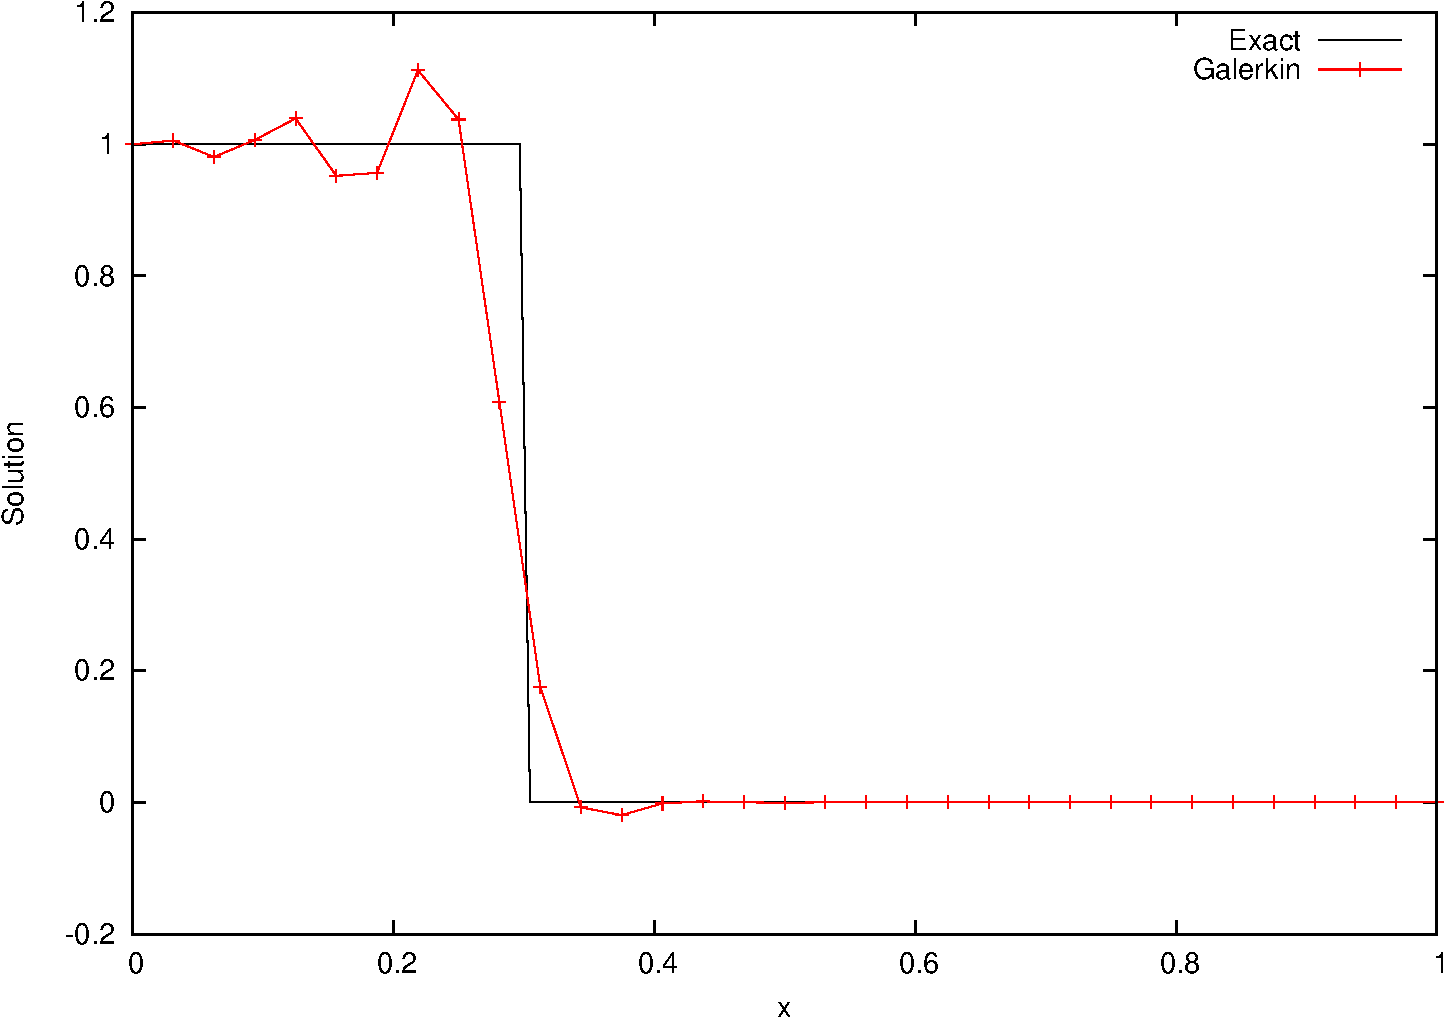
\includegraphics[width=0.7\textwidth]{./figures/advection_Galerkin.pdf}
   \end{center}
\end{itemize}

\end{frame}
%%%%%%%%%%%%%%%%%%%%%%%%%%%%%%%%%%%%%%%%%%%%%%%%%%%%%%%%%%%%%%%%%%%%%%%%%%%%%%%%%
\subsection{Objectives}
\begin{frame}
\frametitle{Objectives}

\begin{itemize}
   \item The objectives of the research are the following:
   \begin{itemize}
      \item \textbf{Accurately solve conservation law problems} using the
         continuous finite element method (CFEM).
      \begin{itemize}
         \item Scheme to be presented is 2nd order-accurate in space (for smooth
            problems).
      \end{itemize}
      \item \textbf{Prevent spurious oscillations}.
      \begin{itemize}
	 \item Scheme to be presented is not proven to be completely immune to any
            spurious oscillations but shows good results in practice.
      \end{itemize}
      \item \textbf{Prevent negativities} for physically non-negative quantities.
      \begin{itemize}
         \item Scheme to be presented is guaranteed to be positivity-preserving.
      \end{itemize}
   \end{itemize}
\end{itemize}

\end{frame}
%%%%%%%%%%%%%%%%%%%%%%%%%%%%%%%%%%%%%%%%%%%%%%%%%%%%%%%%%%%%%%%%%%%%%%%%%%%%%%%%%
\subsection{Previous Work}
\begin{frame}
\frametitle{Previous Work}

\begin{itemize}
  \item Guermond has addressed these objectives for general nonlinear scalar
    conservation laws using explicit temporal discretizations:
    \[
      \pd{u}{t} + \nabla\cdot\mathbf{f}(u) = 0
    \]
  \item We extend these techniques to include a reaction term and source term
    and to use implicit and steady-state temporal discretizations:
    \[
      \pd{u}{t} + \nabla\cdot\mathbf{f}(u) + \sigma u = q
    \]
\end{itemize}

\end{frame}
%%%%%%%%%%%%%%%%%%%%%%%%%%%%%%%%%%%%%%%%%%%%%%%%%%%%%%%%%%%%%%%%%%%%%%%%%%%%%%%%%
\subsection{Outline}
\begin{frame}
\frametitle{Outline}

\begin{itemize}
   \item Presentation of scheme for simple case:
   \begin{itemize}
      \item Problem formulation
      \item Monotone low-order scheme
      \item High-order entropy viscosity scheme
      \item FCT scheme
   \end{itemize}
   \item Results
   \item Implementation in \texttt{deal.II}
   \item Conclusions
\end{itemize}

\end{frame}
%%%%%%%%%%%%%%%%%%%%%%%%%%%%%%%%%%%%%%%%%%%%%%%%%%%%%%%%%%%%%%%%%%%%%%%%%%%%%%%%%
\section{Methodology}
\subsection{Problem Formulation}
\begin{frame}
\frametitle{Problem Formulation}

\begin{itemize}
   \item Scalar linear conservation law model:
   \begin{align}
      &\pd{u}{t} + \nabla\cdot(\mathbf{v}u\xt)
      + \sigma(\x)u\xt = q\xt\\
      &\sigma(\x)\ge 0,\qquad q\xt\ge 0\nonumber
   \end{align}
   \item Define problem by providing initial conditions and some boundary
      condition, such as Dirichlet:
   \begin{equation}
      u(\x,0) = u^0(\x) \quad \forall \x\in \mathcal{D}
   \end{equation}
   \begin{equation}
      u\xt = u^{inc}(\x) \quad \forall \x\in \partial \mathcal{D}^{inc}
   \end{equation}
   \item CFEM solution:
   \begin{equation}
      u_h\xt = \sum\limits_{j=1}^N U_j(t) \varphi_j(\x),
      \quad \varphi_j(\x)\in P^1_h
   \end{equation}
\end{itemize}

\end{frame}
%%%%%%%%%%%%%%%%%%%%%%%%%%%%%%%%%%%%%%%%%%%%%%%%%%%%%%%%%%%%%%%%%%%%%%%%%%%%%%%%%
\subsection{Time Discretization}
\begin{frame}
\frametitle{Time Discretization}

\begin{itemize}
   \item Simplest time discretization is forward Euler (FE), which gives the
      discrete system
   \begin{equation}
      \M^C\frac{\U^{n+1}-\U^n}{\dt} + \A\U^n = \b^n
   \end{equation}
   \begin{equation}
      M\ij^C \equiv \int\limits_{S\ij}\varphi_i(\x) \varphi_j(\x) d\x
   \end{equation}
   \begin{equation}
      A\ij \equiv \int\limits_{S\ij}\left(
      \mathbf{v}\cdot\nabla\varphi_j(\x) +
		\sigma(\x)\varphi_j(\x)\right)\varphi_i(\x) d\x
   \end{equation}
   \begin{equation}
      b_i^n \equiv \int\limits_{S_i} q(\x,t^n)\varphi_i(\x) d\x
   \end{equation}
\end{itemize}

\end{frame}
%%%%%%%%%%%%%%%%%%%%%%%%%%%%%%%%%%%%%%%%%%%%%%%%%%%%%%%%%%%%%%%%%%%%%%%%%%%%%%%%%
\subsection{FCT Scheme Overview}
\begin{frame}
\frametitle{Flux Corrected Transport (FCT) Scheme}
\framesubtitle{Introduction}

\begin{itemize}
   \item Initially developed in 1973 for finite difference discretizations of
      transport/conservation law problems and recently applied to finite element
      method.
   \item Works by adding conservative fluxes to satisfy physical bounds on the
      solution.
   \item Employs a high-order scheme and a low-order, monotone scheme.
   \item Defines a \emph{correction}, or \emph{antidiffusion}, flux, which
      when added to the low-order scheme, produces the high-order scheme
      solution.
   \item Limits this correction flux to enforce the physical bounds imposed.
\end{itemize}

\end{frame}
%%%%%%%%%%%%%%%%%%%%%%%%%%%%%%%%%%%%%%%%%%%%%%%%%%%%%%%%%%%%%%%%%%%%%%%%%%%%%%%%%
\subsection{Low-Order Scheme}
\begin{frame}
\frametitle{Low-Order Scheme}
\framesubtitle{Definition}

\begin{itemize}
   \item To get the low-order scheme, one does the following:
   \begin{itemize}
      \item Lumps the mass matrix: $\M^C \rightarrow \M^L$.
      \item Adds a low-order diffusion operator: $\A \rightarrow \A+\D^L$.
   \end{itemize}
   \item This gives the following, where $\U^{L,n+1}$ is the low-order solution:
   \begin{equation}
      \M^L\frac{\U^{L,n+1}-\U^n}{\dt} + (\A + \D^L)\U^n = \b^n
   \end{equation}
   \item The diffusion matrix $\D^L$ is assembled elementwise, where $K$
      denotes an element, using a local bilinear form $b_K$ and a
      local low-order viscosity $\nu_K^L$:
   \begin{equation}
      D\ij^L = \sum\limits_{K\subset S\ij}\nu_K^L b_K(\varphi_j,\varphi_i)
   \end{equation}
\end{itemize}

\end{frame}
%%%%%%%%%%%%%%%%%%%%%%%%%%%%%%%%%%%%%%%%%%%%%%%%%%%%%%%%%%%%%%%%%%%%%%%%%%%%%%%%%
\begin{frame}
\frametitle{Low-Order Scheme}
\framesubtitle{Local Bilinear Form}

\begin{itemize}
   \item The local bilinear form is defined as follows, where $|K|$ denotes
      the volume of element $K$, $\mathcal{I}(K)$ is the set of indices
      corresponding to degrees of freedom with nonempty support on $K$, and
      $n_K$ is the cardinality of this set.
   \begin{equation}
      b_K(\varphi_j, \varphi_i) \equiv \left\{\begin{array}{l l}
         -\frac{1}{n_K - 1}|K| & i\ne j, \quad i,j\in \mathcal{I}(K)\\
         |K|                   & i = j,  \quad i,j\in \mathcal{I}(K)\\
         0                     & i\notin\mathcal{I}(K)\,|\, j\notin\mathcal{I}(K)
      \end{array}\right.
   \end{equation}
   \item Some properties that result from this definition:
   \begin{equation}
      \sum\limits_j b_K(\varphi_j, \varphi_i) = 0
   \end{equation}
   \begin{equation}
      b_K(\varphi_i, \varphi_i) > 0
   \end{equation}
\end{itemize}

\end{frame}
%%%%%%%%%%%%%%%%%%%%%%%%%%%%%%%%%%%%%%%%%%%%%%%%%%%%%%%%%%%%%%%%%%%%%%%%%%%%%%%%%
\begin{frame}
\frametitle{Low-Order Scheme}
\framesubtitle{Low-Order Viscosity}

\begin{itemize}
   \item The low-order viscosity is defined as
   \begin{equation}
      \nu_K^L \equiv \max\limits_{i\ne j\in \mathcal{I}(K)}\frac{\max(0,A\ij)}
      {-\sum\limits_{T\subset S\ij} b_T(\varphi_j, \varphi_i)}
   \end{equation}
   \item This definition is designed to be the smallest number such that the
      following is guaranteed:
   \begin{equation}
      D^L\ij \leq -A\ij, \quad j\ne i
   \end{equation}
   \item This is used to guarantee that the low-order steady-state matrix
      $\A^L=\A+\D^L$ is an M-matrix, i.e., a \emph{monotone} matrix:
      $\A^L\U \ge 0\Rightarrow \U\ge 0$.
\end{itemize}

\end{frame}
%%%%%%%%%%%%%%%%%%%%%%%%%%%%%%%%%%%%%%%%%%%%%%%%%%%%%%%%%%%%%%%%%%%%%%%%%%%%%%%%%
\begin{frame}
\frametitle{Low-Order Scheme}
\framesubtitle{Discrete Maximum Principle}

\begin{itemize}
   \item In addition to guaranteeing monotonicity and positivity, the low-order
      viscous terms guarantee the following discrete maximum principle (DMP),
      where $U^n_{\substack{\max\\\min},i} =
      \substack{\max\\\min\limits_{j\in\mathcal{I}(S_i)}}U^n_j$:
      \begin{equation}
         W_i^-\leq
         U_i^{L,n+1}\leq
         W_i^+\qquad\forall i
      \end{equation}
      \begin{equation}
         W_i^\pm \equiv U_{\substack{\max\\\min},i}^n\left(
         1-\frac{\dt}{M_{i,i}^L}
         \sum\limits_j A\ij^L\right)
         + \frac{\Delta t}{M_{i,i}^L}b_i^n
      \end{equation}
   \item For example, when there is no reaction term or source term, this reduces
      to the following DMP, which implies the scheme is local extremum
      diminishing (LED):
      \begin{equation}
         U^n_{\min,i}\leq
         U_i^{L,n+1}\leq
         U^n_{\max,i}\qquad\forall i
      \end{equation}
\end{itemize}

\end{frame}
%%%%%%%%%%%%%%%%%%%%%%%%%%%%%%%%%%%%%%%%%%%%%%%%%%%%%%%%%%%%%%%%%%%%%%%%%%%%%%%%%
\begin{frame}
\frametitle{Low-Order Scheme}
\framesubtitle{Results Example}

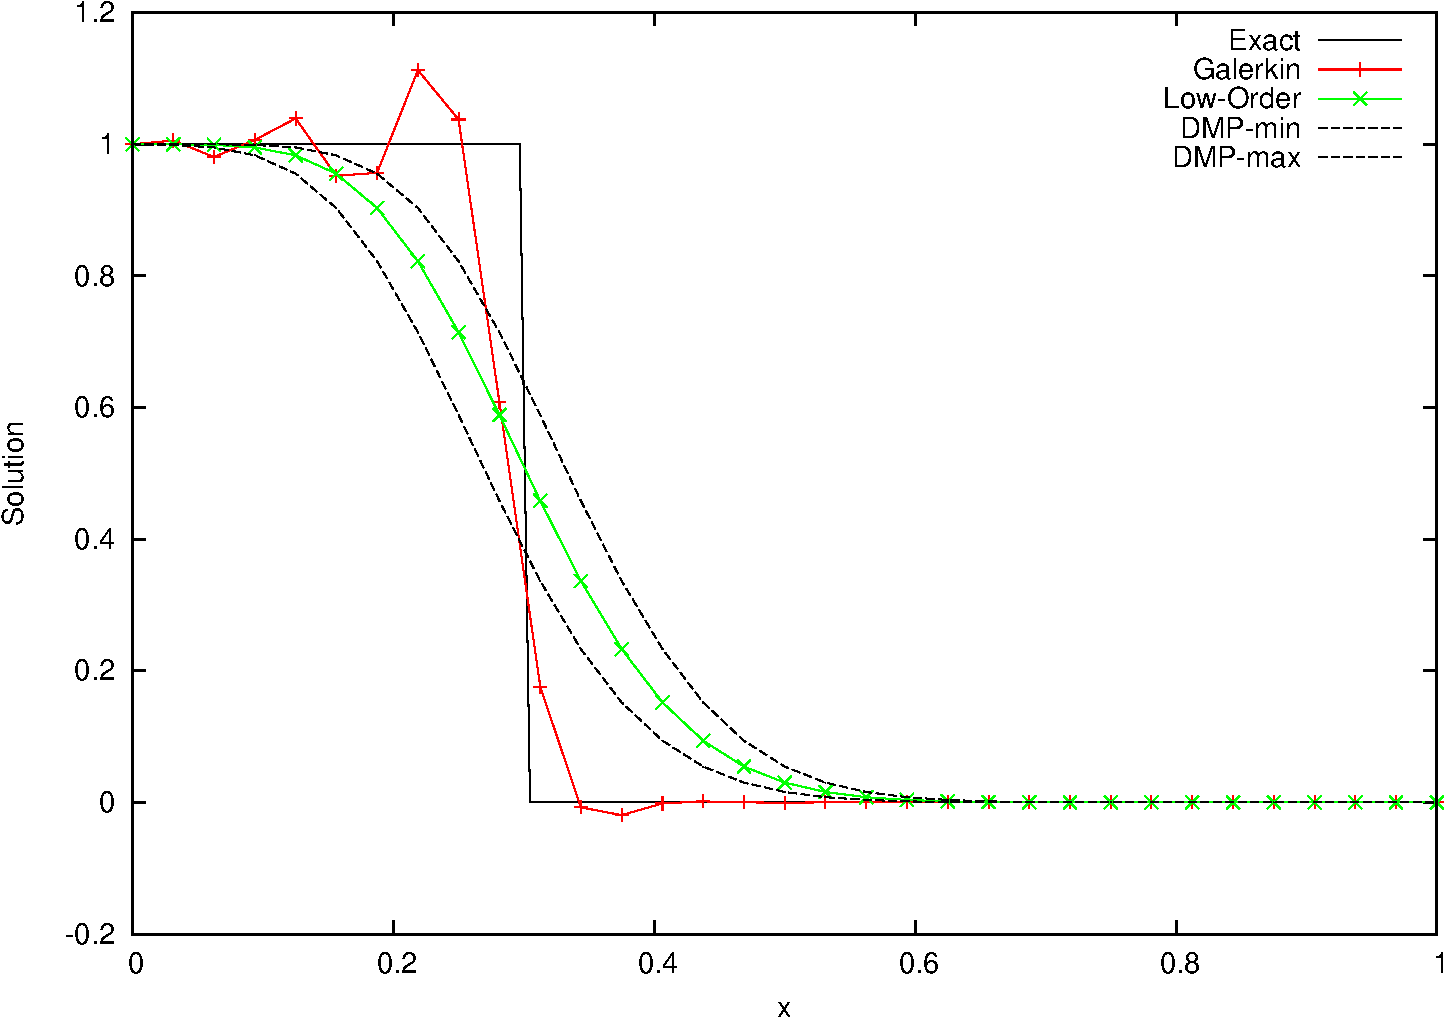
\includegraphics[width=\textwidth]{./figures/advection_low_order.pdf}

\end{frame}
%%%%%%%%%%%%%%%%%%%%%%%%%%%%%%%%%%%%%%%%%%%%%%%%%%%%%%%%%%%%%%%%%%%%%%%%%%%%%%%%%
\subsection{High-Order Scheme}
\begin{frame}
\frametitle{Entropy Viscosity Scheme}
\framesubtitle{Introduction}

\begin{itemize}
   \item The standard Galerkin CFEM weak solution is not unique. Even with
      FCT, it would not necessarily converge to the correct, physical
      weak solution, i.e., the \emph{entropy} solution.
   \item To converge to the entropy solution, one must ensure that an entropy
      inequality is satisfied:
      \begin{equation}
         R(u) \equiv \pd{\eta(u)}{t} + \nabla\cdot\mathbf{f}^\eta(u) \leq 0
      \end{equation}
      for any convex entropy $\eta(u)$ and corresponding entropy flux
      $\mathbf{f}^\eta(u)$.
   \item This \emph{entropy residual} $R(u)$ measures entropy production;
      where it is positive, the inequality is violated, so the residual
      should be decreased somehow.
   \item To enforce the inequality, the entropy viscosity method adds
      viscosity in proportion to local entropy production, thus decreasing
      local entropy.
\end{itemize}

\end{frame}
%%%%%%%%%%%%%%%%%%%%%%%%%%%%%%%%%%%%%%%%%%%%%%%%%%%%%%%%%%%%%%%%%%%%%%%%%%%%%%%%%
\begin{frame}
\frametitle{Entropy Viscosity Scheme}
\framesubtitle{Entropy Viscosity Definition}

\begin{itemize}
   \item One chooses a convex entropy function $\eta(u)$ such
   as $\eta(u)=\frac{1}{2}u^2$ and manipulates the
   conservation law equation to get an entropy residual:
   \begin{equation}
      R(u) = \pd{\eta}{t}
      + \frac{d\eta}{du}\left(\nabla\cdot(\mathbf{v}u)
      + \sigma u 
      - q \right)
   \end{equation}
   \item Viscosity is set to be proportional to a linear combination
      of the local entropy residual $R_K(u) = \left\|R(u)\right\|_{L^\infty(K)}$
      and entropy jumps $J_F(u)$ across the faces:
      \begin{equation}
         \nu^{\eta}_K \propto c_R R_K(u_h)
         + c_J\max\limits_{F\in\partial K}J_F(u_h)
      \end{equation}
   \item In practice, the entropy viscosity becomes the following, where the
      denominator is just a normalization constant:
      \begin{equation}
         \nu^{\eta}_K = \frac{c_R R_K(u_h)
         + c_J\max\limits_{F\in\partial K}J_F(u_h)}
         {\|\eta(u_h)-\bar{\eta}(u_h)\|_{L^\infty(\mathcal{D})}}
      \end{equation}
\end{itemize}
   
\end{frame}
%%%%%%%%%%%%%%%%%%%%%%%%%%%%%%%%%%%%%%%%%%%%%%%%%%%%%%%%%%%%%%%%%%%%%%%%%%%%%%%%%
\begin{frame}
\frametitle{Entropy Viscosity Scheme}
\framesubtitle{High-Order Scheme}

\begin{itemize}
   \item The high-order viscosity does not need to be any greater than the
      low-order viscosity:
      \begin{equation}
         \nu^{H,n}_K = \min(\nu^{L}_K,\nu^{\eta,n}_K)
      \end{equation}
   \item For the high-order scheme, the mass matrix is not modified; the
      only change is the addition of the high-order diffusion operator
      $\D^{H,n}$: $\A \rightarrow \A + \D^{H,n}$:
      \begin{equation}
         \M^C\frac{\U^{H,n+1}-\U^n}{\dt} + (\A + \D^{H,n})\U^n = \b^n
      \end{equation}
   \item The high-order diffusion matrix is computed just as the low-order
      counterpart, except that $\nu^{H,n}_K$ is used instead of $\nu^{L}_K$:
      \begin{equation}
         D\ij^{H,n} = \sum\limits_{K\subset S\ij}\nu_K^{H,n}
            b_K(\varphi_j,\varphi_i)
      \end{equation}
\end{itemize}

\end{frame}
%%%%%%%%%%%%%%%%%%%%%%%%%%%%%%%%%%%%%%%%%%%%%%%%%%%%%%%%%%%%%%%%%%%%%%%%%%%%%%%%%
\begin{frame}
\frametitle{High-Order Scheme}
\framesubtitle{Results Example}

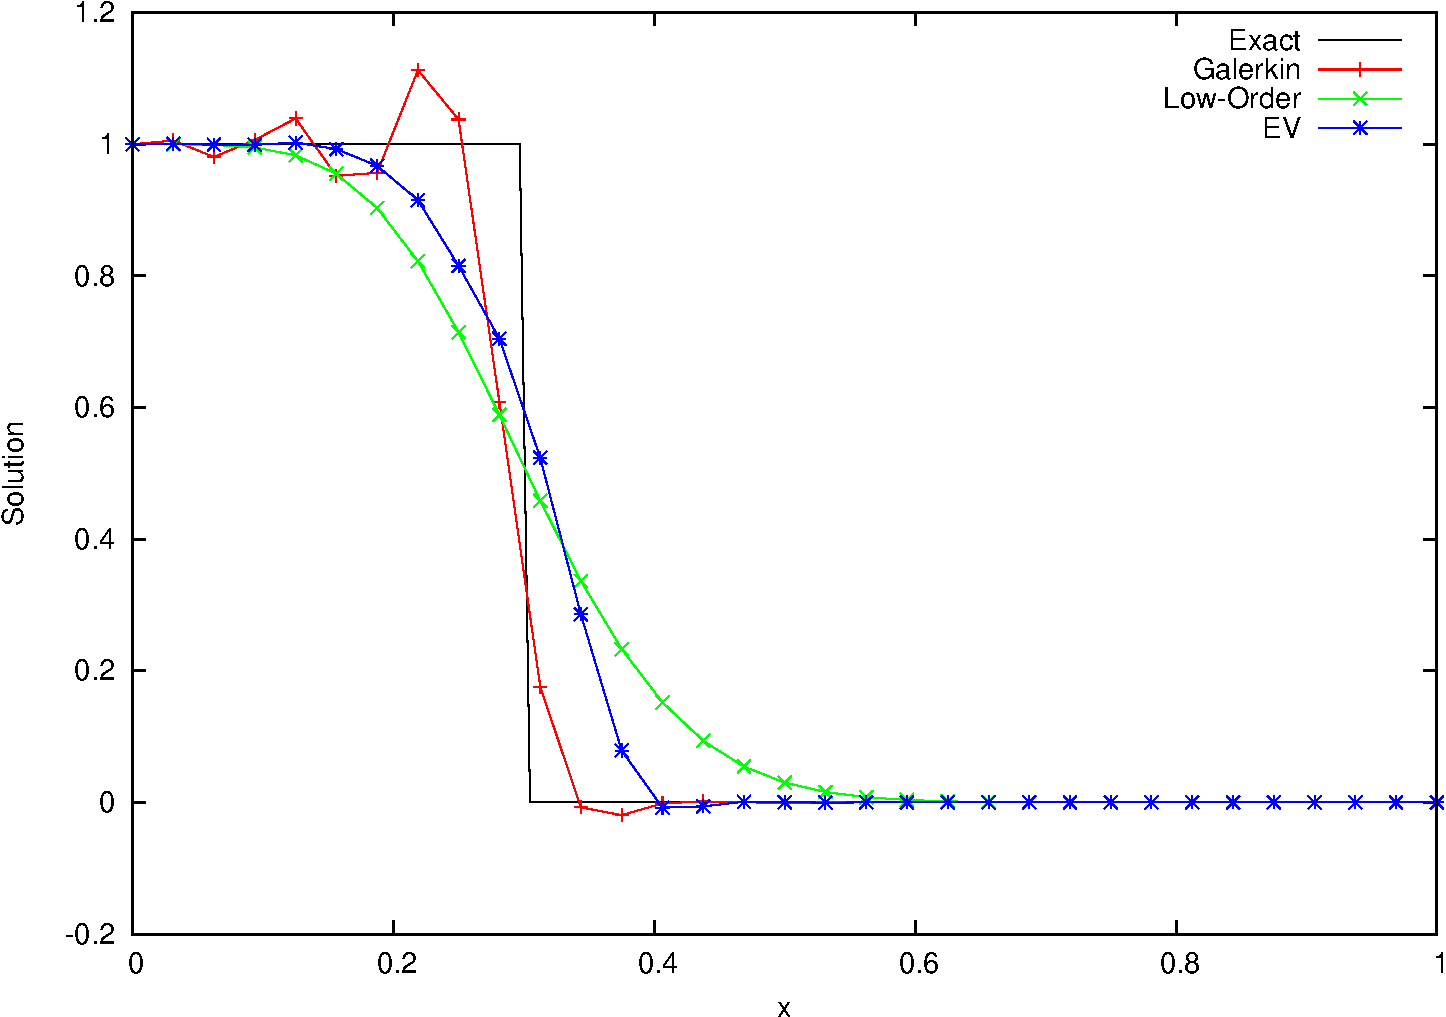
\includegraphics[width=\textwidth]{./figures/advection_high_order.pdf}

\end{frame}
%%%%%%%%%%%%%%%%%%%%%%%%%%%%%%%%%%%%%%%%%%%%%%%%%%%%%%%%%%%%%%%%%%%%%%%%%%%%%%%%%
\subsection{FCT Scheme}
\begin{frame}
\frametitle{Flux Corrected Transport (FCT) Scheme}
\framesubtitle{Correction Flux Definition}

\begin{itemize}
   \item Recall that FCT defines antidiffusive correction fluxes
      from a low-order, monotone scheme to a high-order scheme. Calling
      these fluxes $\f$, this gives
      \begin{equation}
         \M^L\frac{\U^{H,n+1}-\U^n}{\dt}+(\A+\D^L)\U^n = \b^n + \f
      \end{equation}
   \item Subtracting the high-order scheme equation from this gives the
      definition of $\f$:
      \begin{equation}
         \f \equiv -(\M^C-\M^L)\frac{\U^{H,n+1}-\U^n}{\dt} +(\D^L-\D^{H,n})\U^n
      \end{equation}
   \item Decomposing $\f$ into internodal fluxes
      $F\ij$ such that $f_i = \sum_j F\ij$, where $\Delta_{j,i}[\mathbf{y}]$
      denotes $y_j - y_i$:
   \begin{equation}
      F\ij = -M\ij^C\Delta_{j,i}\left[\frac{\U^{H,n+1}-\U^n}{\Delta t}\right]
      + (D\ij^L-D\ij^{H,n})\Delta_{j,i}[\U^n]
   \end{equation}
\end{itemize}

\end{frame}
%%%%%%%%%%%%%%%%%%%%%%%%%%%%%%%%%%%%%%%%%%%%%%%%%%%%%%%%%%%%%%%%%%%%%%%%%%%%%%%%%
\begin{frame}
\frametitle{Flux Corrected Transport (FCT) Scheme}
\framesubtitle{FCT Overview}

\begin{itemize}
   \item Recall that the objective of FCT is to limit these antidiffusive
      fluxes to enforce some physical bounds.
   \item The chosen bounds take the form of the DMP satisfied by the
      low-order scheme:
      \begin{equation}
         W_i^-\leq
         U_i^{n+1}\leq
         W_i^+\qquad\forall i
      \end{equation}
   \item This is achieved by applying a limiting coefficient $L\ij$ to each
      internodal flux $F\ij$:
      \begin{equation}
         \M^L\frac{\U^{n+1}-\U^n}{\dt} + \A^L\U^n = \b + \L\cdot\F
      \end{equation}
   \item Each limiting coefficient is between zero and unity: $0\leq L\ij\leq 1$.
   \begin{itemize}
      \item If all $L\ij$ are zero, then the low-order scheme is produced.
      \item If all $L\ij$ are one, then the high-order scheme is produced.
   \end{itemize}
\end{itemize}

\end{frame}
%%%%%%%%%%%%%%%%%%%%%%%%%%%%%%%%%%%%%%%%%%%%%%%%%%%%%%%%%%%%%%%%%%%%%%%%%%%%%%%%%
\begin{frame}
\frametitle{Flux Corrected Transport (FCT) Scheme}
\framesubtitle{Limiting Coefficients Definition}

\begin{itemize}
   \item The enforced bounds can be rearranged to bound the limited flux sums
      with bounds which we call $Q_i^\pm$:
      \begin{equation}
         Q^-_i \leq \sum\limits_j L\ij F\ij \leq Q^+_i
      \end{equation}
      \begin{equation}
         F_i^- \equiv \sum\limits_{j:F\ij<0} F\ij \qquad
         F_i^+ \equiv \sum\limits_{j:F\ij>0} F\ij
      \end{equation}
      \begin{equation}
         L_i^\pm \equiv\left\{
            \begin{array}{l l}
               1                                          & F_i^\pm = 0\\
               \min\left(1,\frac{Q_i^\pm}{F_i^\pm}\right) & F_i^\pm \ne 0
            \end{array}
            \right.
      \end{equation}
      \begin{equation}
         L\ij \equiv\left\{
            \begin{array}{l l}
               \min(L_i^+,L_j^-) & F_{i,j} \geq 0\\
               \min(L_i^-,L_j^+) & F_{i,j} < 0
            \end{array}
            \right.
      \end{equation}
\end{itemize}

\end{frame}
%%%%%%%%%%%%%%%%%%%%%%%%%%%%%%%%%%%%%%%%%%%%%%%%%%%%%%%%%%%%%%%%%%%%%%%%%%%%%%%%%
\begin{frame}
\frametitle{Flux Corrected Transport (FCT) Scheme}
\framesubtitle{Results Example}

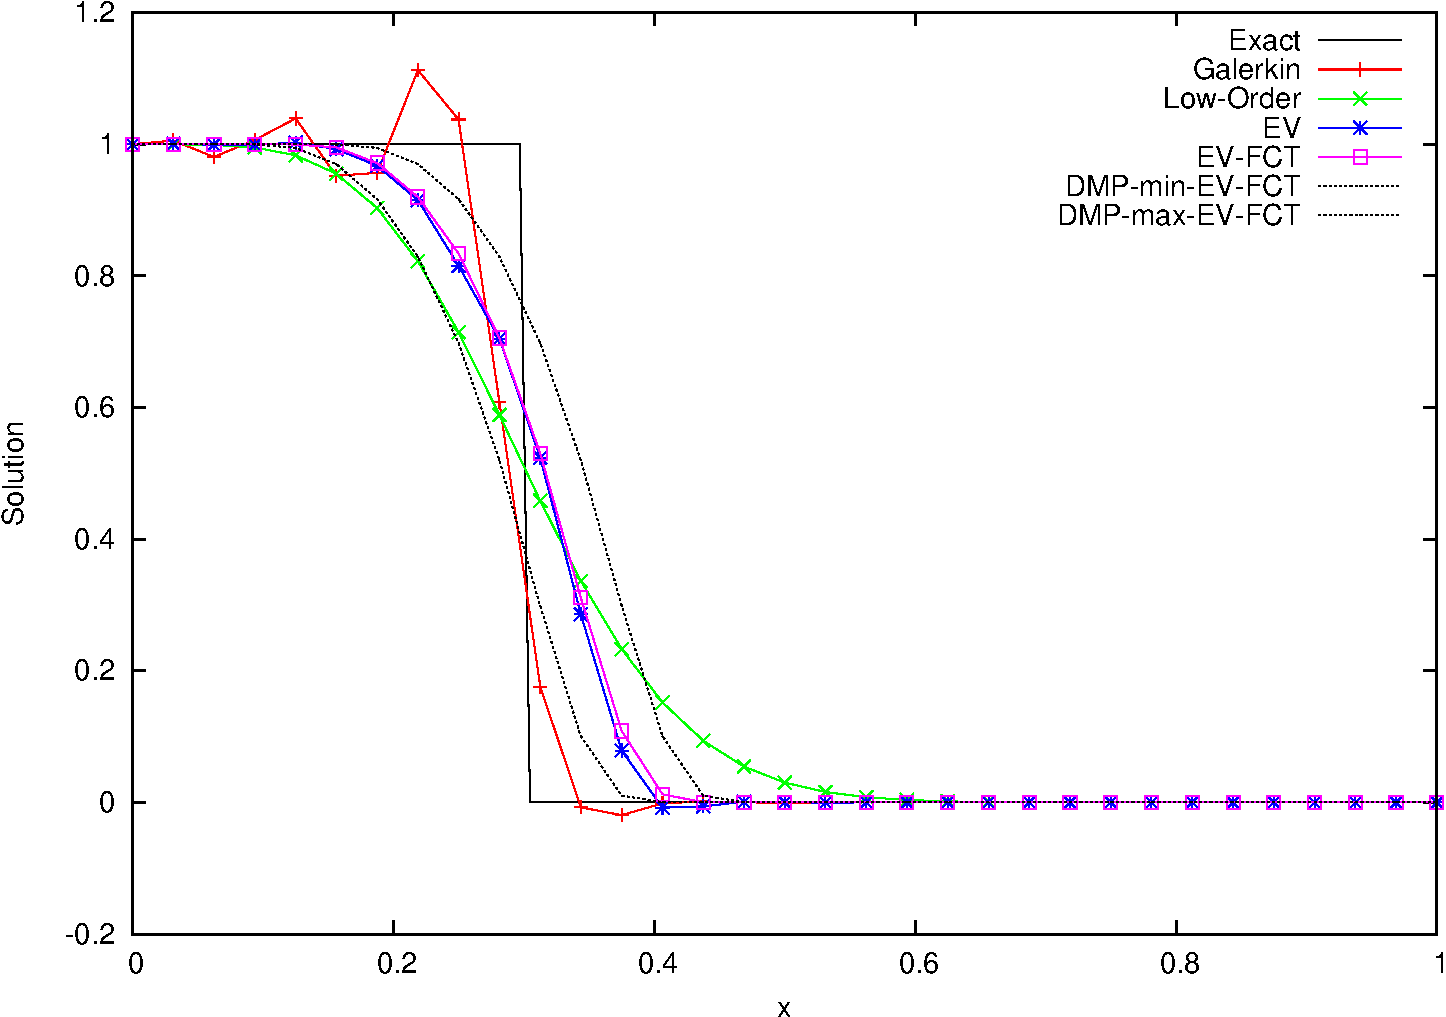
\includegraphics[width=\textwidth]{./figures/advection_FCT.pdf}

\end{frame}
%%%%%%%%%%%%%%%%%%%%%%%%%%%%%%%%%%%%%%%%%%%%%%%%%%%%%%%%%%%%%%%%%%%%%%%%%%%%%%%%%
\section{Results}
\begin{frame}
\frametitle{Results}
\framesubtitle{1-D Source Problem Results}

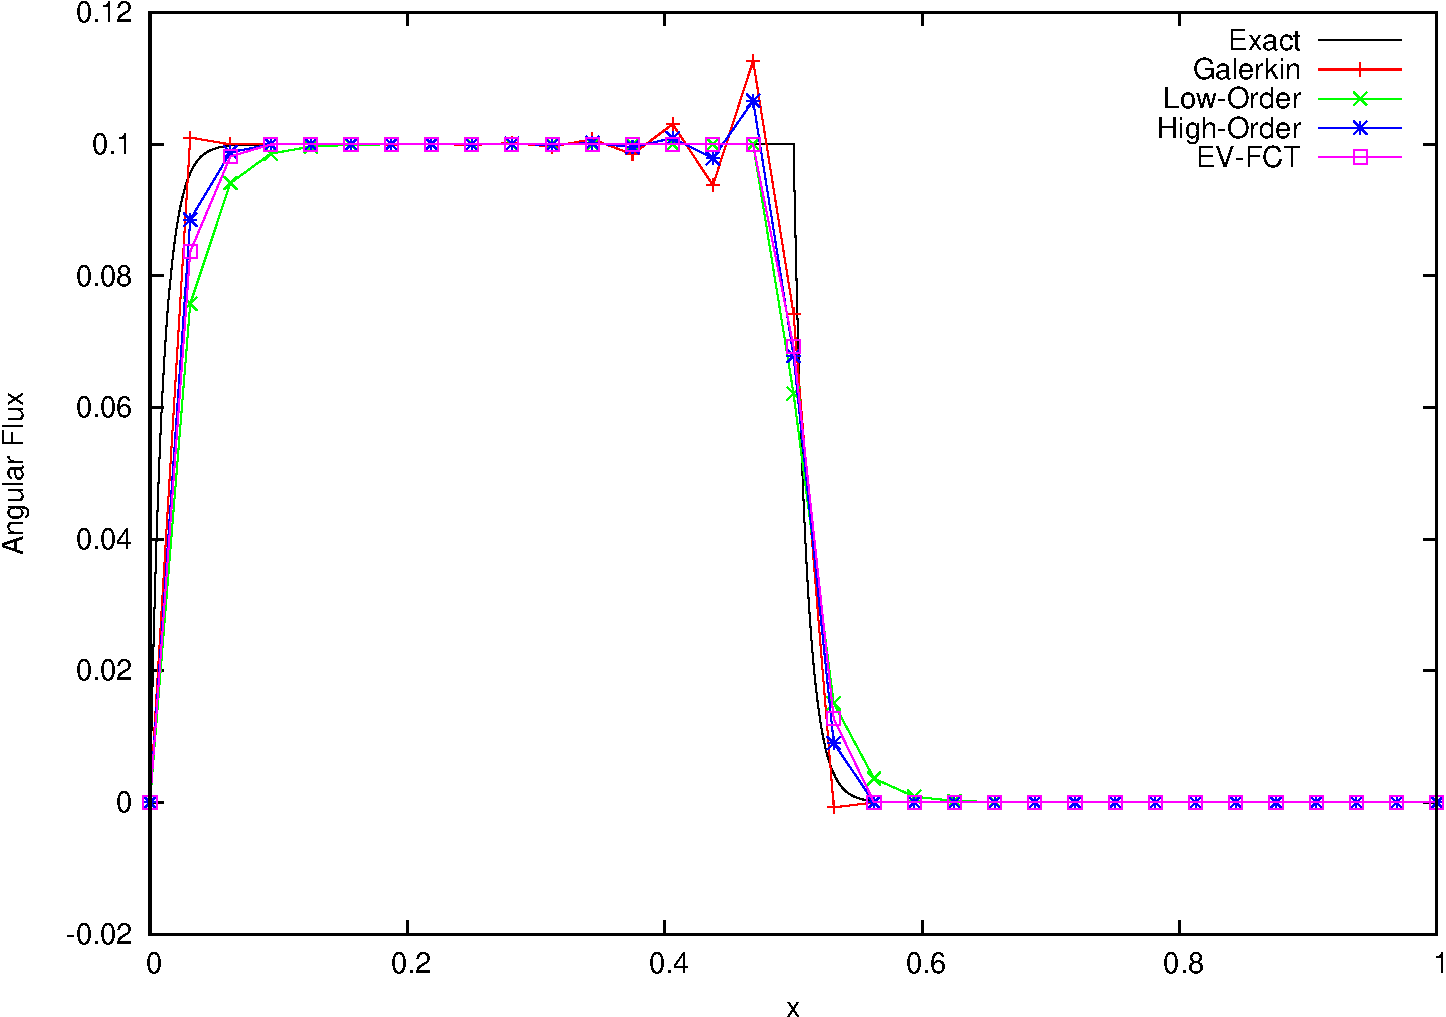
\includegraphics[width=\textwidth]{./figures/solutions_source_FE.pdf}

\end{frame}
%%%%%%%%%%%%%%%%%%%%%%%%%%%%%%%%%%%%%%%%%%%%%%%%%%%%%%%%%%%%%%%%%%%%%%%%%%%%%%%%%
\begin{frame}
\frametitle{Results}
\framesubtitle{2-D Void-to-Absorber Problem Results}

\begin{figure}[h]
   \centering
   \begin{subfigure}{0.3\textwidth}
      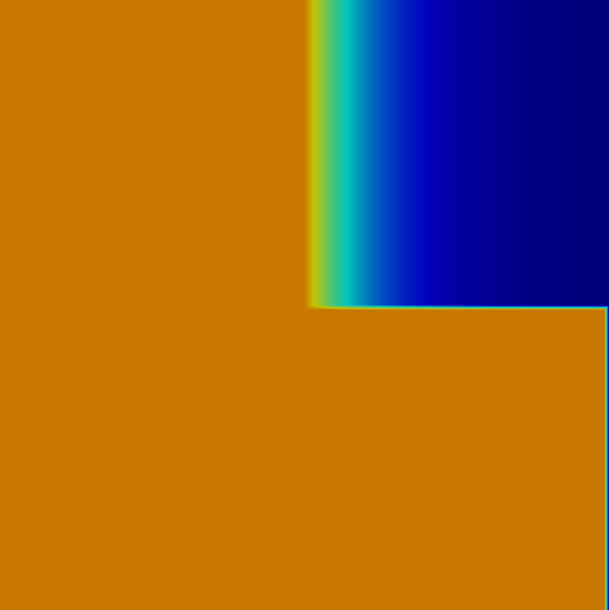
\includegraphics[width=\textwidth]{./figures/exact.png}
      \caption{Exact}
   \end{subfigure}
   \begin{subfigure}{0.3\textwidth}
      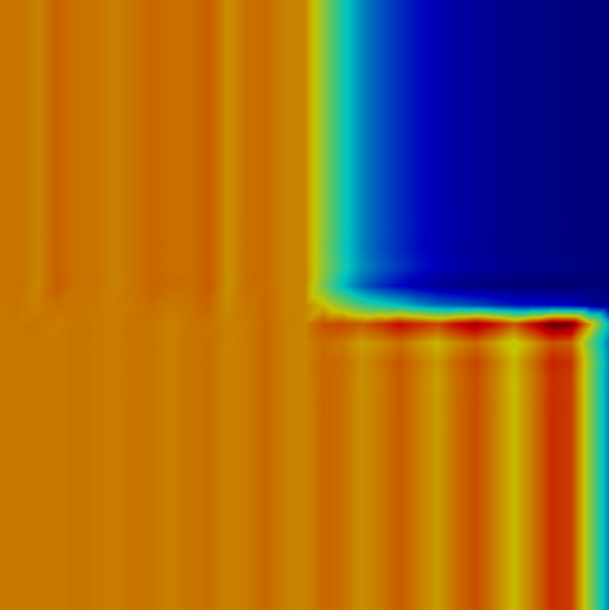
\includegraphics[width=\textwidth]{./figures/Gal.png}
      \caption{Galerkin}
   \end{subfigure}
   \begin{subfigure}{0.3\textwidth}
      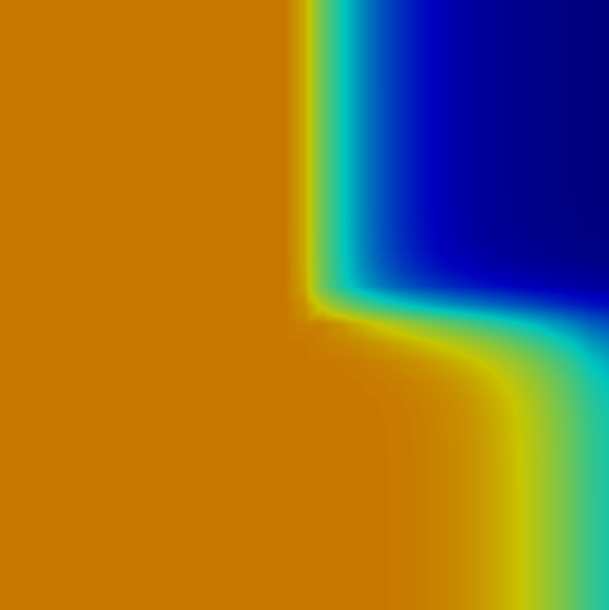
\includegraphics[width=\textwidth]{./figures/GalFCT.png}
      \caption{Galerkin-FCT}
   \end{subfigure}
   \begin{subfigure}{0.3\textwidth}
      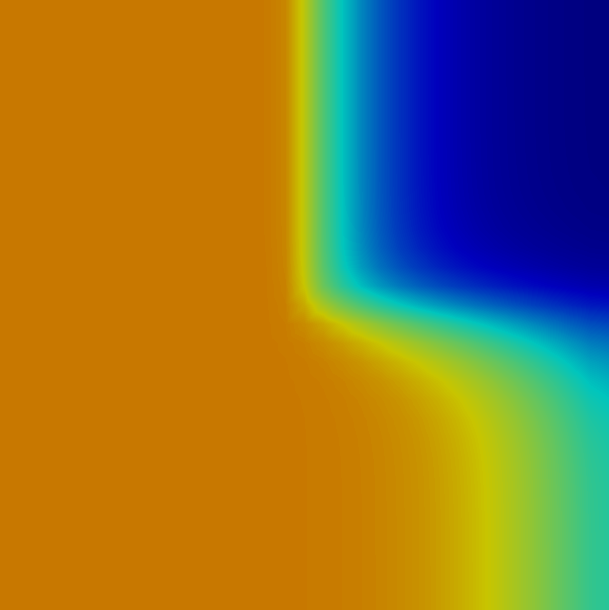
\includegraphics[width=\textwidth]{./figures/low.png}
      \caption{Low-order}
   \end{subfigure}
   \begin{subfigure}{0.3\textwidth}
      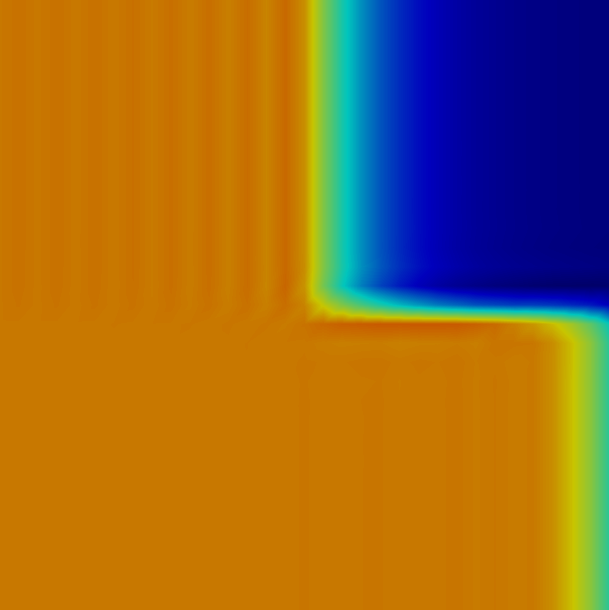
\includegraphics[width=\textwidth]{./figures/EV.png}
      \caption{EV}
   \end{subfigure}
   \begin{subfigure}{0.3\textwidth}
      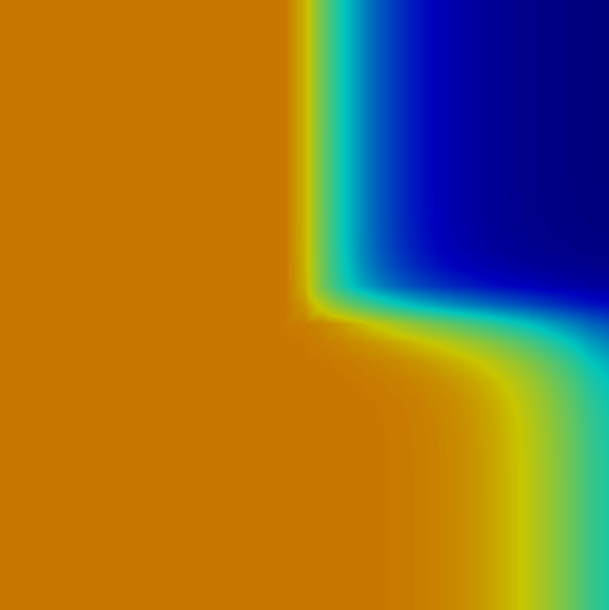
\includegraphics[width=\textwidth]{./figures/EVFCT.png}
      \caption{EV-FCT}
   \end{subfigure}
\end{figure}

\end{frame}
%%%%%%%%%%%%%%%%%%%%%%%%%%%%%%%%%%%%%%%%%%%%%%%%%%%%%%%%%%%%%%%%%%%%%%%%%%%%%%%%%
\begin{frame}
\frametitle{Results}
\framesubtitle{1-D Smooth Problem Convergence Results (Using FE)}

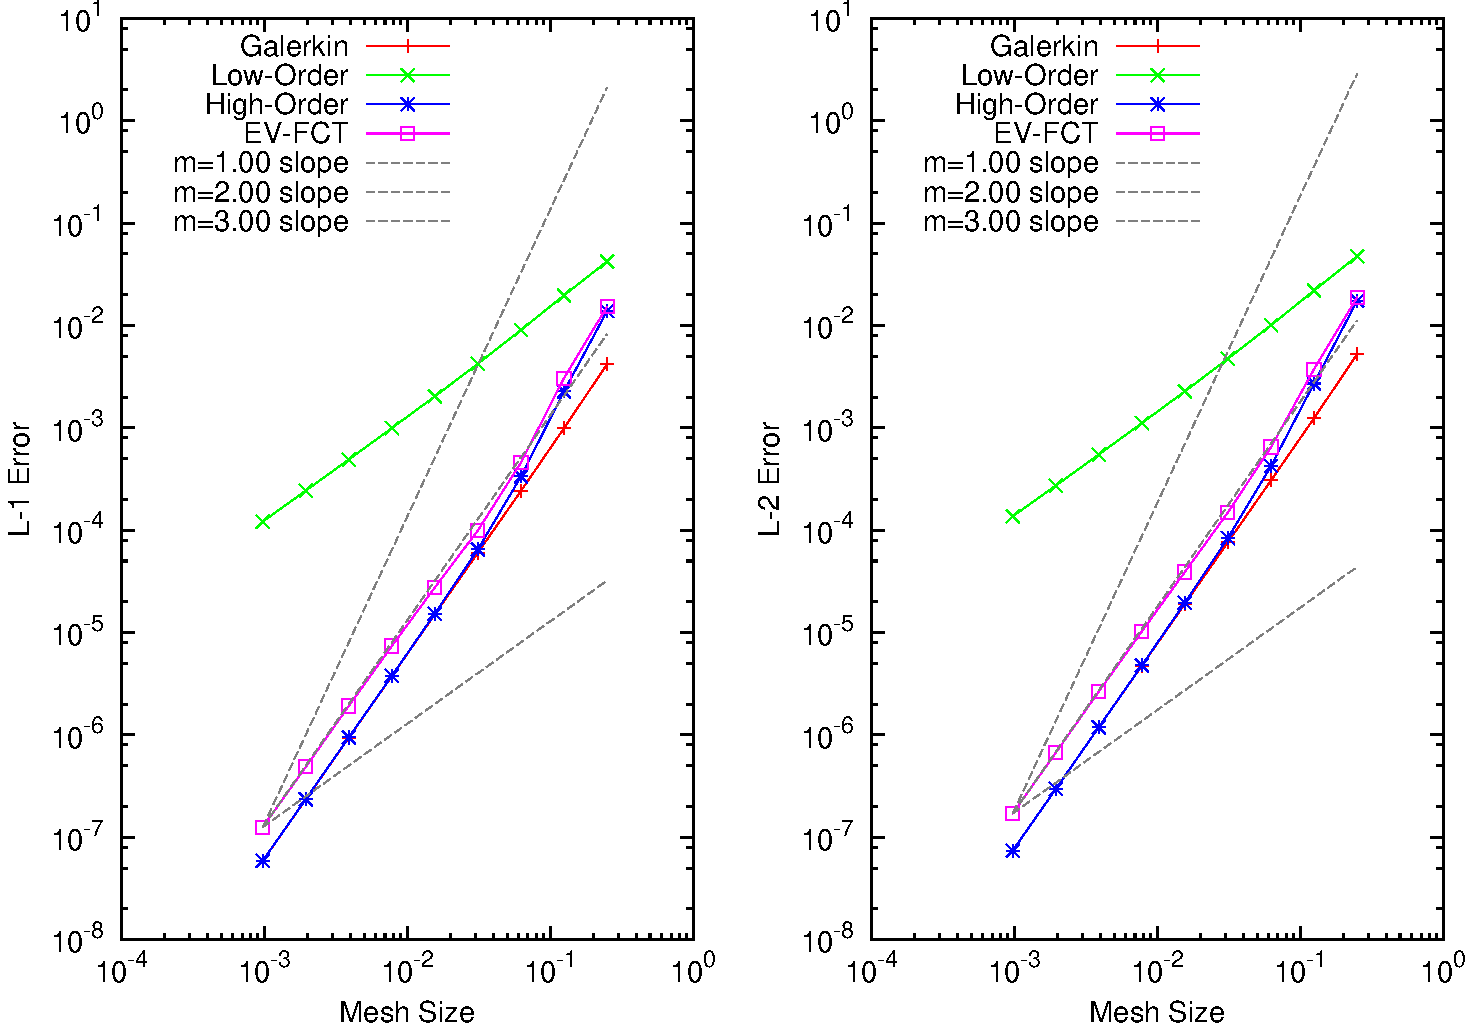
\includegraphics[width=\textwidth]{./figures/convergence_smooth_FE.pdf}

\end{frame}
%%%%%%%%%%%%%%%%%%%%%%%%%%%%%%%%%%%%%%%%%%%%%%%%%%%%%%%%%%%%%%%%%%%%%%%%%%%%%%%%%
\begin{frame}
\frametitle{Results}
\framesubtitle{1-D Non-smooth Problem Convergence Results (Using SSPRK33)}

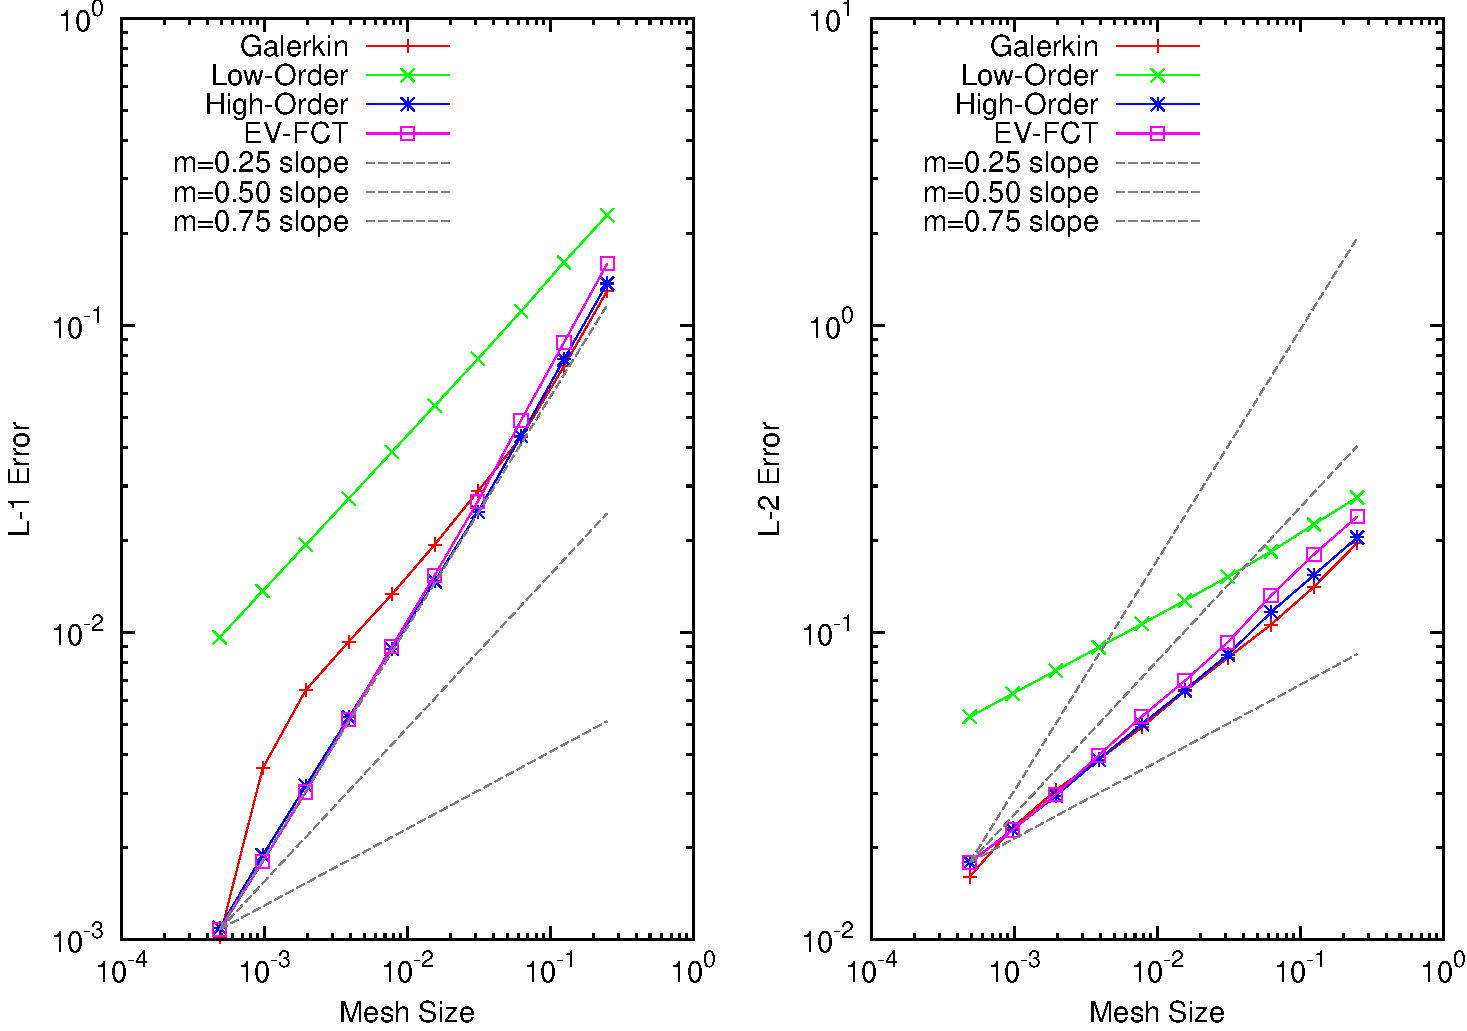
\includegraphics[width=\textwidth]{./figures/convergence_absorber_SSPRK33.pdf}

\end{frame}
%%%%%%%%%%%%%%%%%%%%%%%%%%%%%%%%%%%%%%%%%%%%%%%%%%%%%%%%%%%%%%%%%%%%%%%%%%%%%%%%%
\section{Implementation}
\begin{frame}
\frametitle{Implementation}
\framesubtitle{FCT Implementation Overview}

\begin{itemize}
   \item Summary of steps necessary for FCT scheme:
      \begin{enumerate}
         \item Assemble $\M^C$, $\M^L$, $\A$, $\D^L$, $\D^{H,n}$ (if using EV), $\b$
         \item Compute high-order solution $\U^{H,n+1}$
         \item Compute antidiffusive fluxes $F\ij,\quad\forall j\ne i
            \in\mathcal{I}(S_i)$
         \item Compute DMP bounds $W_i^\pm$
            \begin{itemize}
               \item Need to compute $U_{\substack{\max\\\min},i}$
            \end{itemize}
         \item Compute limiting coefficients $L\ij$
         \item Solve FCT system:
            \begin{equation}
               \M^L\frac{\U^{n+1}-\U^n}{\dt} + \A^L\U^n = \b + \L\cdot\F
            \end{equation}
      \end{enumerate}
\end{itemize}

\end{frame}
%%%%%%%%%%%%%%%%%%%%%%%%%%%%%%%%%%%%%%%%%%%%%%%%%%%%%%%%%%%%%%%%%%%%%%%%%%%%%%%%%
\begin{frame}
\frametitle{Implementation}
\framesubtitle{Determining Overlapping Supports}

\begin{itemize}
   \item Most steps standard, but some steps require algebraic operations
      not typical in FEM computations.
   \item Need to be able to determine $j\in\mathcal{I}(S_i)$.
      Some approaches:
      \begin{itemize}
         \item If sparse matrix class provides function to extract
            a row's entries and corresponding indices, this indicates
            $j\in\mathcal{I}(S_i)$. For instance, do this with $\M^C$.
         \item Since linear FEM, know that only adjacent, i.e., ``connected''
            nodes can share support:
            \[i \mbox{ adjacent } j\Rightarrow j\in\mathcal{I}(S_i),\quad
               i\in\mathcal{I}(S_j)\]
            \item Thus one can loop over these ``edges'', i.e., pairs of nodes
            \item This is particularly useful for computing $F\ij$, since it
               is skew symmetric
      \end{itemize}
\end{itemize}

\end{frame}
%%%%%%%%%%%%%%%%%%%%%%%%%%%%%%%%%%%%%%%%%%%%%%%%%%%%%%%%%%%%%%%%%%%%%%%%%%%%%%%%%
\begin{frame}[fragile=singleslide]
\frametitle{Implementation}
\framesubtitle{Example: Performing Algebraic (Non-Elementwise) Operations}

\begin{itemize}
   \item The objective is obtain the nonzero entries in a row $i$ of a
     sparse matrix $A$.
\end{itemize}

\lstset{basicstyle=\small\ttfamily,language=C++,frame=single,
  keywordstyle=\color{red}\ttfamily,
  commentstyle=\color{blue}\ttfamily}
\begin{lstlisting}
// get iterators for beginning and end of row
SparseMatrixIterator it     = A.begin(i);
                     it_end = A.end(i);

// compute number of nonzero entries in row
n_nonzero_entries = it_end - it;
row_values .resize(n_nonzero_entries);
row_indices.resize(n_nonzero_entries);

// loop over nonzero entries in row
for (int k = 0; it != it_end; ++it, ++k)
{
  row_values[k]  = it->value();  // get A(i,j)
  row_indices[k] = it->column(); // get j
}
\end{lstlisting}

\end{frame}
%%%%%%%%%%%%%%%%%%%%%%%%%%%%%%%%%%%%%%%%%%%%%%%%%%%%%%%%%%%%%%%%%%%%%%%%%%%%%%%%%
\section{Conclusions}
\begin{frame}
\frametitle{Conclusions}

\begin{itemize}
   \item The CFEM scheme presented for solving conservation law problems is
   \begin{itemize}
      \item 2nd-order-accurate
      \item Positivity-preserving
      \item Monotone
      \item Discrete-maximum-principle preserving
      \item Valid in an arbitrary number of dimensions
      \item Valid for general meshes
   \end{itemize}
   \item Results were shown for the explicit, scalar, linear case. More results
      are in progress.
\end{itemize}

\end{frame}
%%%%%%%%%%%%%%%%%%%%%%%%%%%%%%%%%%%%%%%%%%%%%%%%%%%%%%%%%%%%%%%%%%%%%%%%%%%%%%%%%
\end{document}
